% Options for packages loaded elsewhere
\PassOptionsToPackage{unicode}{hyperref}
\PassOptionsToPackage{hyphens}{url}
%
\documentclass[
]{book}
\usepackage{amsmath,amssymb}
\usepackage{iftex}
\ifPDFTeX
  \usepackage[T1]{fontenc}
  \usepackage[utf8]{inputenc}
  \usepackage{textcomp} % provide euro and other symbols
\else % if luatex or xetex
  \usepackage{unicode-math} % this also loads fontspec
  \defaultfontfeatures{Scale=MatchLowercase}
  \defaultfontfeatures[\rmfamily]{Ligatures=TeX,Scale=1}
\fi
\usepackage{lmodern}
\ifPDFTeX\else
  % xetex/luatex font selection
\fi
% Use upquote if available, for straight quotes in verbatim environments
\IfFileExists{upquote.sty}{\usepackage{upquote}}{}
\IfFileExists{microtype.sty}{% use microtype if available
  \usepackage[]{microtype}
  \UseMicrotypeSet[protrusion]{basicmath} % disable protrusion for tt fonts
}{}
\makeatletter
\@ifundefined{KOMAClassName}{% if non-KOMA class
  \IfFileExists{parskip.sty}{%
    \usepackage{parskip}
  }{% else
    \setlength{\parindent}{0pt}
    \setlength{\parskip}{6pt plus 2pt minus 1pt}}
}{% if KOMA class
  \KOMAoptions{parskip=half}}
\makeatother
\usepackage{xcolor}
\usepackage{color}
\usepackage{fancyvrb}
\newcommand{\VerbBar}{|}
\newcommand{\VERB}{\Verb[commandchars=\\\{\}]}
\DefineVerbatimEnvironment{Highlighting}{Verbatim}{commandchars=\\\{\}}
% Add ',fontsize=\small' for more characters per line
\usepackage{framed}
\definecolor{shadecolor}{RGB}{248,248,248}
\newenvironment{Shaded}{\begin{snugshade}}{\end{snugshade}}
\newcommand{\AlertTok}[1]{\textcolor[rgb]{0.94,0.16,0.16}{#1}}
\newcommand{\AnnotationTok}[1]{\textcolor[rgb]{0.56,0.35,0.01}{\textbf{\textit{#1}}}}
\newcommand{\AttributeTok}[1]{\textcolor[rgb]{0.13,0.29,0.53}{#1}}
\newcommand{\BaseNTok}[1]{\textcolor[rgb]{0.00,0.00,0.81}{#1}}
\newcommand{\BuiltInTok}[1]{#1}
\newcommand{\CharTok}[1]{\textcolor[rgb]{0.31,0.60,0.02}{#1}}
\newcommand{\CommentTok}[1]{\textcolor[rgb]{0.56,0.35,0.01}{\textit{#1}}}
\newcommand{\CommentVarTok}[1]{\textcolor[rgb]{0.56,0.35,0.01}{\textbf{\textit{#1}}}}
\newcommand{\ConstantTok}[1]{\textcolor[rgb]{0.56,0.35,0.01}{#1}}
\newcommand{\ControlFlowTok}[1]{\textcolor[rgb]{0.13,0.29,0.53}{\textbf{#1}}}
\newcommand{\DataTypeTok}[1]{\textcolor[rgb]{0.13,0.29,0.53}{#1}}
\newcommand{\DecValTok}[1]{\textcolor[rgb]{0.00,0.00,0.81}{#1}}
\newcommand{\DocumentationTok}[1]{\textcolor[rgb]{0.56,0.35,0.01}{\textbf{\textit{#1}}}}
\newcommand{\ErrorTok}[1]{\textcolor[rgb]{0.64,0.00,0.00}{\textbf{#1}}}
\newcommand{\ExtensionTok}[1]{#1}
\newcommand{\FloatTok}[1]{\textcolor[rgb]{0.00,0.00,0.81}{#1}}
\newcommand{\FunctionTok}[1]{\textcolor[rgb]{0.13,0.29,0.53}{\textbf{#1}}}
\newcommand{\ImportTok}[1]{#1}
\newcommand{\InformationTok}[1]{\textcolor[rgb]{0.56,0.35,0.01}{\textbf{\textit{#1}}}}
\newcommand{\KeywordTok}[1]{\textcolor[rgb]{0.13,0.29,0.53}{\textbf{#1}}}
\newcommand{\NormalTok}[1]{#1}
\newcommand{\OperatorTok}[1]{\textcolor[rgb]{0.81,0.36,0.00}{\textbf{#1}}}
\newcommand{\OtherTok}[1]{\textcolor[rgb]{0.56,0.35,0.01}{#1}}
\newcommand{\PreprocessorTok}[1]{\textcolor[rgb]{0.56,0.35,0.01}{\textit{#1}}}
\newcommand{\RegionMarkerTok}[1]{#1}
\newcommand{\SpecialCharTok}[1]{\textcolor[rgb]{0.81,0.36,0.00}{\textbf{#1}}}
\newcommand{\SpecialStringTok}[1]{\textcolor[rgb]{0.31,0.60,0.02}{#1}}
\newcommand{\StringTok}[1]{\textcolor[rgb]{0.31,0.60,0.02}{#1}}
\newcommand{\VariableTok}[1]{\textcolor[rgb]{0.00,0.00,0.00}{#1}}
\newcommand{\VerbatimStringTok}[1]{\textcolor[rgb]{0.31,0.60,0.02}{#1}}
\newcommand{\WarningTok}[1]{\textcolor[rgb]{0.56,0.35,0.01}{\textbf{\textit{#1}}}}
\usepackage{longtable,booktabs,array}
\usepackage{calc} % for calculating minipage widths
% Correct order of tables after \paragraph or \subparagraph
\usepackage{etoolbox}
\makeatletter
\patchcmd\longtable{\par}{\if@noskipsec\mbox{}\fi\par}{}{}
\makeatother
% Allow footnotes in longtable head/foot
\IfFileExists{footnotehyper.sty}{\usepackage{footnotehyper}}{\usepackage{footnote}}
\makesavenoteenv{longtable}
\usepackage{graphicx}
\makeatletter
\def\maxwidth{\ifdim\Gin@nat@width>\linewidth\linewidth\else\Gin@nat@width\fi}
\def\maxheight{\ifdim\Gin@nat@height>\textheight\textheight\else\Gin@nat@height\fi}
\makeatother
% Scale images if necessary, so that they will not overflow the page
% margins by default, and it is still possible to overwrite the defaults
% using explicit options in \includegraphics[width, height, ...]{}
\setkeys{Gin}{width=\maxwidth,height=\maxheight,keepaspectratio}
% Set default figure placement to htbp
\makeatletter
\def\fps@figure{htbp}
\makeatother
\usepackage{soul}
\setlength{\emergencystretch}{3em} % prevent overfull lines
\providecommand{\tightlist}{%
  \setlength{\itemsep}{0pt}\setlength{\parskip}{0pt}}
\setcounter{secnumdepth}{5}
\usepackage{booktabs}
\ifLuaTeX
  \usepackage{selnolig}  % disable illegal ligatures
\fi
\usepackage[]{natbib}
\bibliographystyle{plainnat}
\IfFileExists{bookmark.sty}{\usepackage{bookmark}}{\usepackage{hyperref}}
\IfFileExists{xurl.sty}{\usepackage{xurl}}{} % add URL line breaks if available
\urlstyle{same}
\hypersetup{
  pdftitle={Informe de resumen de clases},
  hidelinks,
  pdfcreator={LaTeX via pandoc}}

\title{Informe de resumen de clases}
\author{true}
\date{2023-10-26}

\usepackage{amsthm}
\newtheorem{theorem}{Theorem}[chapter]
\newtheorem{lemma}{Lemma}[chapter]
\newtheorem{corollary}{Corollary}[chapter]
\newtheorem{proposition}{Proposition}[chapter]
\newtheorem{conjecture}{Conjecture}[chapter]
\theoremstyle{definition}
\newtheorem{definition}{Definition}[chapter]
\theoremstyle{definition}
\newtheorem{example}{Example}[chapter]
\theoremstyle{definition}
\newtheorem{exercise}{Exercise}[chapter]
\theoremstyle{definition}
\newtheorem{hypothesis}{Hypothesis}[chapter]
\theoremstyle{remark}
\newtheorem*{remark}{Remark}
\newtheorem*{solution}{Solution}
\begin{document}
\maketitle

{
\setcounter{tocdepth}{1}
\tableofcontents
}
\hypertarget{motivaciuxf3n}{%
\chapter*{Motivación}\label{motivaciuxf3n}}
\addcontentsline{toc}{chapter}{Motivación}

Fortalecer habilidades profesionales para incrementar capacidad operativa de una organización social

\hypertarget{uso}{%
\section*{Uso}\label{uso}}
\addcontentsline{toc}{section}{Uso}

Revision de los temas vistos en todas las sesiones de entrenamiento en R para data science

\hypertarget{render-book}{%
\section*{Render book}\label{render-book}}
\addcontentsline{toc}{section}{Render book}

You can render the HTML version of this example book without changing anything:

\begin{enumerate}
\def\labelenumi{\arabic{enumi}.}
\item
  Find the \textbf{Build} pane in the RStudio IDE, and
\item
  Click on \textbf{Build Book}, then select your output format, or select ``All formats'' if you'd like to use multiple formats from the same book source files.
\end{enumerate}

Or build the book from the R console:

\begin{Shaded}
\begin{Highlighting}[]
\NormalTok{bookdown}\SpecialCharTok{::}\FunctionTok{render\_book}\NormalTok{()}
\end{Highlighting}
\end{Shaded}

To render this example to PDF as a \texttt{bookdown::pdf\_book}, you'll need to install XeLaTeX. You are recommended to install TinyTeX (which includes XeLaTeX): \url{https://yihui.org/tinytex/}.

\hypertarget{preview-book}{%
\section*{Preview book}\label{preview-book}}
\addcontentsline{toc}{section}{Preview book}

As you work, you may start a local server to live preview this HTML book. This preview will update as you edit the book when you save individual .Rmd files. You can start the server in a work session by using the RStudio add-in ``Preview book'', or from the R console:

\begin{Shaded}
\begin{Highlighting}[]
\NormalTok{bookdown}\SpecialCharTok{::}\FunctionTok{serve\_book}\NormalTok{()}
\end{Highlighting}
\end{Shaded}

\hypertarget{introduccion-a-markdown-en-rstudio}{%
\chapter*{Introduccion a Markdown en RStudio}\label{introduccion-a-markdown-en-rstudio}}
\addcontentsline{toc}{chapter}{Introduccion a Markdown en RStudio}

n esta clase, aprenderemos los conceptos básicos de RStudio y Markdown. Markdown es una sintaxis ligera y fácil de usar que te permite darle formato el texto de manera sencilla y eficiente en tus informes y documentos.

\hypertarget{quuxe9-es-markdown}{%
\section*{¿Qué es Markdown?}\label{quuxe9-es-markdown}}
\addcontentsline{toc}{section}{¿Qué es Markdown?}

Markdown es un lenguaje de marcado ligero que permite dar formato al texto de manera simple. Es ampliamente utilizado en la generación de informes, documentación, blogs y más. Markdown es ideal para crear contenido de manera rápida y sin complicaciones

\hypertarget{ventajas-de-markdown}{%
\subsection*{Ventajas de Markdown}\label{ventajas-de-markdown}}
\addcontentsline{toc}{subsection}{Ventajas de Markdown}

\begin{itemize}
\tightlist
\item
  \textbf{Sencillo}: La sintaxis de Markdown es fácil de aprender y usar
\item
  \textbf{Legible}: Los documentos Markdown son legibles en formato plano
\item
  \textbf{Portátil}: Podemos usarla en varios editores de texto
\item
  \textbf{Versátil}: Es compatible con HTML, y esto permite combinarlo con otros elementos
\item
  \textbf{Reproducible}: Facilita la reproducción de resultados y la colaboración en proyectos.
\end{itemize}

\hypertarget{sintaxis-basica-de-markdown}{%
\section*{Sintaxis basica de Markdown}\label{sintaxis-basica-de-markdown}}
\addcontentsline{toc}{section}{Sintaxis basica de Markdown}

Podemos crear encabezados utilizando el simbolo \texttt{\#}. Cuantos mas \texttt{\#}, más pequeño va a ser el encabezado

\hypertarget{ejemplos}{%
\subsection*{Ejemplos:}\label{ejemplos}}
\addcontentsline{toc}{subsection}{Ejemplos:}

\begin{itemize}
\item ~
  \hypertarget{encabezados-1}{%
  \chapter{Encabezados 1}\label{encabezados-1}}
\item ~
  \hypertarget{encabezados-2}{%
  \section{Encabezados 2}\label{encabezados-2}}
\item ~
  \hypertarget{encabezados-3}{%
  \subsection{Encabezados 3}\label{encabezados-3}}
\end{itemize}

\hypertarget{dar-formato-al-texto}{%
\subsection*{Dar formato al texto}\label{dar-formato-al-texto}}
\addcontentsline{toc}{subsection}{Dar formato al texto}

Puede saplicar formato al texto de la siguiente manera:

\begin{itemize}
\tightlist
\item
  \texttt{**Negrilla**}: \textbf{texto}
\item
  \texttt{\_Cursiva\_} o \texttt{*Cursiva*}: \emph{texto} o \emph{texto}
\item
  \texttt{\textasciitilde{}\textasciitilde{}Tachado\textasciitilde{}\textasciitilde{}}: \st{texto}
\end{itemize}

\hypertarget{crear-listas}{%
\subsection*{Crear Listas}\label{crear-listas}}
\addcontentsline{toc}{subsection}{Crear Listas}

Creacion de listas ordenadas y no ordenadas

\textbf{Listas no ordenadas}
- Elemento 1

\begin{itemize}
\item
  Elemento 2

  \begin{itemize}
  \item
    Elemento 2.1
  \item
    Elemento 2.2
  \end{itemize}
\item
  Elemento 3

  \begin{itemize}
  \tightlist
  \item
    Elemento 3.1
  \end{itemize}
\end{itemize}

\textbf{Listas ordenadas}

Si lo que queremos es crear una lista ordenada, debemos introducir un número con un punto directamente.

\begin{enumerate}
\def\labelenumi{\arabic{enumi}.}
\tightlist
\item
  Primer elemento
\item
  Segundo elemento
\item
  Tercer elemento
\end{enumerate}

\hypertarget{recursos-adicionales}{%
\section*{Recursos adicionales}\label{recursos-adicionales}}
\addcontentsline{toc}{section}{Recursos adicionales}

\href{https://github.com/adam-p/markdown-here/wiki/Markdown-Cheatsheet}{\textbf{Markdown Cheat Sheet}}

\href{https://guides.github.com/features/mastering-markdown/}{\textbf{Markdown Guide}}

\href{https://www.markdowntutorial.com}{\textbf{Markdown Tutorial}}

\textbf{Construccion de informes en R}
\textbf{Desarrollado por: \href{https://linkedin.com/in/carmurrain}{Crispthofer Rincon}}
\emph{\textbf{2023}}

\hypertarget{inclusiuxf3n-de-cuxf3digo-en-informes-rmarkdown}{%
\chapter*{Inclusión de código en Informes RMarkdown}\label{inclusiuxf3n-de-cuxf3digo-en-informes-rmarkdown}}
\addcontentsline{toc}{chapter}{Inclusión de código en Informes RMarkdown}

Exploraremos como incluir y ejecutar código en informes RMArkdown. Se aprendera sobre los ``chunks'' de código y cómo cargar y examinar una base de datos en RMarkdown

\hypertarget{chunks-de-cuxf3digo}{%
\section*{Chunks de código}\label{chunks-de-cuxf3digo}}
\addcontentsline{toc}{section}{Chunks de código}

Los ``chunks'' de código son bloques de código que puedes incluir en tu informe. Puede ser ejecutado y mostrar los resultados directamente en el informe.

\begin{Shaded}
\begin{Highlighting}[]
\CommentTok{\# Ejemplo de chunk en R}
\NormalTok{x }\OtherTok{\textless{}{-}} \DecValTok{1}\SpecialCharTok{:}\DecValTok{5}
\NormalTok{y }\OtherTok{\textless{}{-}} \DecValTok{1}\SpecialCharTok{:}\DecValTok{12}
\NormalTok{z }\OtherTok{\textless{}{-}} \DecValTok{1}\SpecialCharTok{:}\DecValTok{20}
\NormalTok{sum\_x }\OtherTok{\textless{}{-}} \FunctionTok{sum}\NormalTok{(x)}
\NormalTok{sum\_x}
\end{Highlighting}
\end{Shaded}

\begin{verbatim}
## [1] 15
\end{verbatim}

\begin{Shaded}
\begin{Highlighting}[]
\NormalTok{mean\_x }\OtherTok{\textless{}{-}} \FunctionTok{mean}\NormalTok{(x)}
\NormalTok{mean\_x}
\end{Highlighting}
\end{Shaded}

\begin{verbatim}
## [1] 3
\end{verbatim}

\begin{Shaded}
\begin{Highlighting}[]
\NormalTok{sum\_y }\OtherTok{\textless{}{-}} \FunctionTok{sum}\NormalTok{(y)}
\NormalTok{sum\_y}
\end{Highlighting}
\end{Shaded}

\begin{verbatim}
## [1] 78
\end{verbatim}

\begin{Shaded}
\begin{Highlighting}[]
\NormalTok{mean\_y }\OtherTok{\textless{}{-}} \FunctionTok{mean}\NormalTok{(y)}
\NormalTok{mean\_y}
\end{Highlighting}
\end{Shaded}

\begin{verbatim}
## [1] 6.5
\end{verbatim}

\begin{Shaded}
\begin{Highlighting}[]
\NormalTok{sum\_z }\OtherTok{\textless{}{-}} \FunctionTok{sum}\NormalTok{(z)}
\NormalTok{sum\_z}
\end{Highlighting}
\end{Shaded}

\begin{verbatim}
## [1] 210
\end{verbatim}

\begin{Shaded}
\begin{Highlighting}[]
\NormalTok{mean\_z }\OtherTok{\textless{}{-}} \FunctionTok{mean}\NormalTok{(z)}
\NormalTok{mean\_z}
\end{Highlighting}
\end{Shaded}

\begin{verbatim}
## [1] 10.5
\end{verbatim}

\hypertarget{carga-y-muestra-de-una-base-de-datos-db}{%
\section*{Carga y muestra de una Base de datos (DB)}\label{carga-y-muestra-de-una-base-de-datos-db}}
\addcontentsline{toc}{section}{Carga y muestra de una Base de datos (DB)}

Para cargar una DB en Markdown, primero debemos asegurar tener la biblioteca adecuada, instalada. Se usara la biblioteca \texttt{readxl} para cargar la DB que están en un archivo excell (\texttt{.xls} o \texttt{.xls})

\begin{Shaded}
\begin{Highlighting}[]
\CommentTok{\# Ejemplo de creación de archivo de excell con R}

\NormalTok{class2\_data }\OtherTok{\textless{}{-}} \FunctionTok{data.frame}\NormalTok{(}
  \AttributeTok{Name =} \FunctionTok{c}\NormalTok{(}
    \StringTok{"Luis"}\NormalTok{, }\StringTok{"Maria"}\NormalTok{, }\StringTok{"Xavier"}\NormalTok{, }
    \StringTok{"Laura"}\NormalTok{, }\StringTok{"Alberto"}\NormalTok{, }\StringTok{"Felipe"}\NormalTok{,}
    \StringTok{"Augusto"}\NormalTok{, }\StringTok{"Julio"}\NormalTok{, }\StringTok{"Ximena"}
\NormalTok{    ),}
  \AttributeTok{Age =} \FunctionTok{c}\NormalTok{(}
    \DecValTok{20}\NormalTok{, }\DecValTok{37}\NormalTok{, }\DecValTok{30}\NormalTok{, }\DecValTok{36}\NormalTok{, }\DecValTok{38}\NormalTok{, }\DecValTok{25}\NormalTok{, }\DecValTok{24}\NormalTok{, }\DecValTok{31}\NormalTok{, }\DecValTok{41}
\NormalTok{  ),}
  \AttributeTok{Score =} \FunctionTok{c}\NormalTok{(}
    \DecValTok{90}\NormalTok{, }\DecValTok{87}\NormalTok{, }\DecValTok{85}\NormalTok{, }\DecValTok{88}\NormalTok{, }\DecValTok{89}\NormalTok{, }\DecValTok{90}\NormalTok{, }\DecValTok{91}\NormalTok{, }\DecValTok{91}\NormalTok{, }\DecValTok{75}
\NormalTok{  )}
\NormalTok{)}

\CommentTok{\# Exportar dataframe a un archivo excell}
\FunctionTok{library}\NormalTok{(openxlsx)}

\FunctionTok{write.xlsx}\NormalTok{(class2\_data, }\AttributeTok{file =} \StringTok{"clase\_2\_data.xlsx"}\NormalTok{)}
\end{Highlighting}
\end{Shaded}

\begin{Shaded}
\begin{Highlighting}[]
\CommentTok{\# Verificación de creación de DB}

\NormalTok{data\_class }\OtherTok{\textless{}{-}} \FunctionTok{read.xlsx}\NormalTok{(}\StringTok{"clase\_2\_data.xlsx"}\NormalTok{)}

\FunctionTok{head}\NormalTok{(data\_class)}
\end{Highlighting}
\end{Shaded}

\begin{verbatim}
##      Name Age Score
## 1    Luis  20    90
## 2   Maria  37    87
## 3  Xavier  30    85
## 4   Laura  36    88
## 5 Alberto  38    89
## 6  Felipe  25    90
\end{verbatim}

\begin{Shaded}
\begin{Highlighting}[]
\FunctionTok{tail}\NormalTok{(data\_class)}
\end{Highlighting}
\end{Shaded}

\begin{verbatim}
##      Name Age Score
## 4   Laura  36    88
## 5 Alberto  38    89
## 6  Felipe  25    90
## 7 Augusto  24    91
## 8   Julio  31    91
## 9  Ximena  41    75
\end{verbatim}

\hypertarget{estadisticas-descriptivas}{%
\section*{Estadisticas descriptivas}\label{estadisticas-descriptivas}}
\addcontentsline{toc}{section}{Estadisticas descriptivas}

\begin{Shaded}
\begin{Highlighting}[]
\CommentTok{\# Clacular las estadisticas para variables Age y Score}

\FunctionTok{summary}\NormalTok{(data\_class}\SpecialCharTok{$}\NormalTok{Age)}
\end{Highlighting}
\end{Shaded}

\begin{verbatim}
##    Min. 1st Qu.  Median    Mean 3rd Qu.    Max. 
##   20.00   25.00   31.00   31.33   37.00   41.00
\end{verbatim}

\begin{Shaded}
\begin{Highlighting}[]
\FunctionTok{summary}\NormalTok{(data\_class}\SpecialCharTok{$}\NormalTok{Score)}
\end{Highlighting}
\end{Shaded}

\begin{verbatim}
##    Min. 1st Qu.  Median    Mean 3rd Qu.    Max. 
##   75.00   87.00   89.00   87.33   90.00   91.00
\end{verbatim}

\hypertarget{gruxe1ficos}{%
\section*{Gráficos}\label{gruxe1ficos}}
\addcontentsline{toc}{section}{Gráficos}

\begin{Shaded}
\begin{Highlighting}[]
\CommentTok{\# Crear histograma variable Age}

\FunctionTok{hist}\NormalTok{(}
\NormalTok{  data\_class}\SpecialCharTok{$}\NormalTok{Age,}
  \AttributeTok{main =} \StringTok{"Histograma de Edades"}\NormalTok{,}
  \AttributeTok{xlab =} \StringTok{"Edad"}\NormalTok{, }\AttributeTok{col =} \StringTok{"orange"}
\NormalTok{  )}
\end{Highlighting}
\end{Shaded}

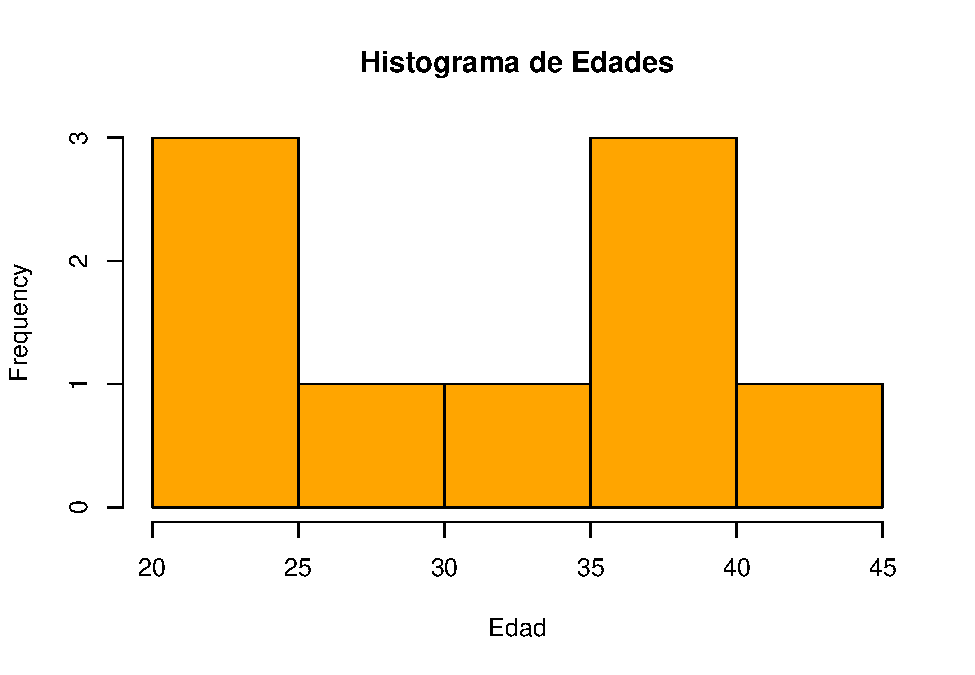
\includegraphics{_main_files/figure-latex/unnamed-chunk-7-1.pdf}

\begin{Shaded}
\begin{Highlighting}[]
\CommentTok{\# Crear gráfico de dispersion Age vs Score}

\FunctionTok{plot}\NormalTok{(}
\NormalTok{  data\_class}\SpecialCharTok{$}\NormalTok{Age, data\_class}\SpecialCharTok{$}\NormalTok{Score,}
  \AttributeTok{xlab =} \StringTok{"Age"}\NormalTok{, }\AttributeTok{ylab =} \StringTok{"Score"}\NormalTok{,}
  \AttributeTok{main =} \StringTok{"Gráfico de dispersión: Age vs Score"}\NormalTok{,}
  \AttributeTok{pch =} \DecValTok{20}
\NormalTok{)}
\end{Highlighting}
\end{Shaded}

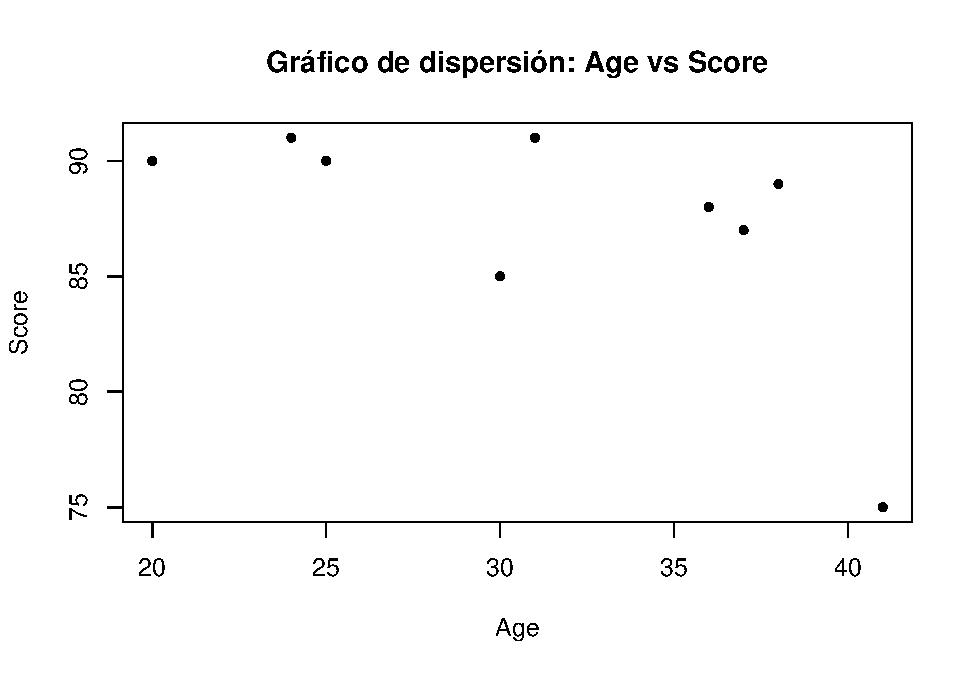
\includegraphics{_main_files/figure-latex/unnamed-chunk-7-2.pdf}

\hypertarget{tablas}{%
\section*{Tablas}\label{tablas}}
\addcontentsline{toc}{section}{Tablas}

\begin{Shaded}
\begin{Highlighting}[]
\FunctionTok{table}\NormalTok{(data\_class}\SpecialCharTok{$}\NormalTok{Name)}
\end{Highlighting}
\end{Shaded}

\begin{verbatim}
## 
## Alberto Augusto  Felipe   Julio   Laura    Luis   Maria  Xavier  Ximena 
##       1       1       1       1       1       1       1       1       1
\end{verbatim}

\hypertarget{introducciuxf3n}{%
\chapter*{Introducción}\label{introducciuxf3n}}
\addcontentsline{toc}{chapter}{Introducción}

Este es un ejemplo de un documento Markdown con varios niveles y subniveles.

\hypertarget{nivel-1}{%
\section*{Nivel 1}\label{nivel-1}}
\addcontentsline{toc}{section}{Nivel 1}

\hypertarget{subnivel-1.1}{%
\subsection*{Subnivel 1.1}\label{subnivel-1.1}}
\addcontentsline{toc}{subsection}{Subnivel 1.1}

Este es un subnivel dentro del Nivel 1.

\hypertarget{subnivel-1.2}{%
\subsection*{Subnivel 1.2}\label{subnivel-1.2}}
\addcontentsline{toc}{subsection}{Subnivel 1.2}

Otro subnivel dentro del Nivel 1.

\hypertarget{nivel-2}{%
\section*{Nivel 2}\label{nivel-2}}
\addcontentsline{toc}{section}{Nivel 2}

\hypertarget{subnivel-2.1}{%
\subsection*{Subnivel 2.1}\label{subnivel-2.1}}
\addcontentsline{toc}{subsection}{Subnivel 2.1}

Dentro del Nivel 2, aquí tenemos un subnivel.

\hypertarget{subsubnivel-2.1.1}{%
\subsubsection*{Subsubnivel 2.1.1}\label{subsubnivel-2.1.1}}
\addcontentsline{toc}{subsubsection}{Subsubnivel 2.1.1}

¡Incluso podemos tener subsubniveles!

\hypertarget{nivel-3}{%
\section*{Nivel 3}\label{nivel-3}}
\addcontentsline{toc}{section}{Nivel 3}

\hypertarget{subnivel-3.1}{%
\subsection*{Subnivel 3.1}\label{subnivel-3.1}}
\addcontentsline{toc}{subsection}{Subnivel 3.1}

Y aquí hay otro nivel 3.

\hypertarget{conclusiuxf3n}{%
\section*{Conclusión}\label{conclusiuxf3n}}
\addcontentsline{toc}{section}{Conclusión}

\hypertarget{footnotes-and-citations}{%
\chapter{Footnotes and citations}\label{footnotes-and-citations}}

\hypertarget{footnotes}{%
\section{Footnotes}\label{footnotes}}

Footnotes are put inside the square brackets after a caret \texttt{\^{}{[}{]}}. Like this one \footnote{This is a footnote.}.

\hypertarget{citations}{%
\section{Citations}\label{citations}}

Reference items in your bibliography file(s) using \texttt{@key}.

For example, we are using the \textbf{bookdown} package \citep{R-bookdown} (check out the last code chunk in index.Rmd to see how this citation key was added) in this sample book, which was built on top of R Markdown and \textbf{knitr} \citep{xie2015} (this citation was added manually in an external file book.bib).
Note that the \texttt{.bib} files need to be listed in the index.Rmd with the YAML \texttt{bibliography} key.

The RStudio Visual Markdown Editor can also make it easier to insert citations: \url{https://rstudio.github.io/visual-markdown-editing/\#/citations}

\hypertarget{blocks}{%
\chapter{Blocks}\label{blocks}}

\hypertarget{equations}{%
\section{Equations}\label{equations}}

Here is an equation.

\begin{equation} 
  f\left(k\right) = \binom{n}{k} p^k\left(1-p\right)^{n-k}
  \label{eq:binom}
\end{equation}

You may refer to using \texttt{\textbackslash{}@ref(eq:binom)}, like see Equation \eqref{eq:binom}.

\hypertarget{theorems-and-proofs}{%
\section{Theorems and proofs}\label{theorems-and-proofs}}

Labeled theorems can be referenced in text using \texttt{\textbackslash{}@ref(thm:tri)}, for example, check out this smart theorem \ref{thm:tri}.

\begin{theorem}
\protect\hypertarget{thm:tri}{}\label{thm:tri}For a right triangle, if \(c\) denotes the \emph{length} of the hypotenuse
and \(a\) and \(b\) denote the lengths of the \textbf{other} two sides, we have
\[a^2 + b^2 = c^2\]
\end{theorem}

Read more here \url{https://bookdown.org/yihui/bookdown/markdown-extensions-by-bookdown.html}.

\hypertarget{callout-blocks}{%
\section{Callout blocks}\label{callout-blocks}}

The R Markdown Cookbook provides more help on how to use custom blocks to design your own callouts: \url{https://bookdown.org/yihui/rmarkdown-cookbook/custom-blocks.html}

\hypertarget{sharing-your-book}{%
\chapter{Sharing your book}\label{sharing-your-book}}

\hypertarget{publishing}{%
\section{Publishing}\label{publishing}}

HTML books can be published online, see: \url{https://bookdown.org/yihui/bookdown/publishing.html}

\hypertarget{pages}{%
\section{404 pages}\label{pages}}

By default, users will be directed to a 404 page if they try to access a webpage that cannot be found. If you'd like to customize your 404 page instead of using the default, you may add either a \texttt{\_404.Rmd} or \texttt{\_404.md} file to your project root and use code and/or Markdown syntax.

\hypertarget{metadata-for-sharing}{%
\section{Metadata for sharing}\label{metadata-for-sharing}}

Bookdown HTML books will provide HTML metadata for social sharing on platforms like Twitter, Facebook, and LinkedIn, using information you provide in the \texttt{index.Rmd} YAML. To setup, set the \texttt{url} for your book and the path to your \texttt{cover-image} file. Your book's \texttt{title} and \texttt{description} are also used.

This \texttt{gitbook} uses the same social sharing data across all chapters in your book- all links shared will look the same.

Specify your book's source repository on GitHub using the \texttt{edit} key under the configuration options in the \texttt{\_output.yml} file, which allows users to suggest an edit by linking to a chapter's source file.

Read more about the features of this output format here:

\url{https://pkgs.rstudio.com/bookdown/reference/gitbook.html}

Or use:

\begin{Shaded}
\begin{Highlighting}[]
\NormalTok{?bookdown}\SpecialCharTok{::}\NormalTok{gitbook}
\end{Highlighting}
\end{Shaded}


  \bibliography{book.bib,packages.bib}

\end{document}
